\section{Realer Speicher}

\subsection{Monoprogrammierung}

Bei der Monoprogrammierung kann nur 1 Programm gleichzeitig ausgeführt werden.
OS und Programm teilen sich den Speicher auf.

\subsection{Speicherpartitionierung}

Speicher wird in $n$ fixe Partitionen aufgeteilt. Die Aufteilung kann nach
Systemstart nicht mehr geändert werden. Prozesse werden auf die vorhandenen
Partitionen aufgeteilt.

\begin{figure}[H]

	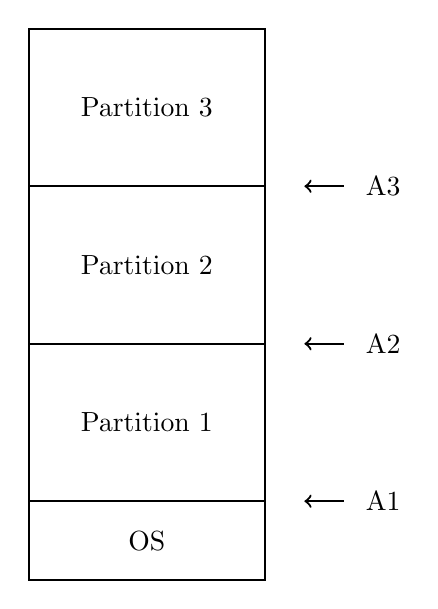
\begin{tikzpicture}
		% Main shape
		\draw[thick] (0,0) rectangle (3,7);
		\draw[thick] (0,1) -- (3,1);
		\draw[thick] (0,3) -- (3,3);
		\draw[thick] (0,5) -- (3,5);
		% Labels
		\node at (1.5,0.5) {OS};
		\node at (1.5,2) {Partition 1};
		\node at (1.5,4) {Partition 2};
		\node at (1.5,6) {Partition 3};
		% Adress-Pfeile
		\draw[thick, ->] (4,1) -- (3.5,1);
		\node at (4.5,1) {A1};
		\draw[thick, ->] (4,3) -- (3.5,3);
		\node at (4.5,3) {A2};
		\draw[thick, ->] (4,5) -- (3.5,5);
		\node at (4.5,5) {A3};
	\end{tikzpicture}

	\caption{Drei Partitionen fixer Grösse mit den Startadressen A1 - A3.}

\end{figure}

\subsubsection{Partitionszuteilung}

\textbf{Gemeinsame Warteschlange}

\begin{itemize}
	\item ...
\end{itemize}

\textbf{Warteschlange pro Partition}

\begin{itemize}
	\item Speichernutzung gut...
\end{itemize}

\subsubsection{Probleme}

\begin{itemize}
	\item Relokation: Programme werden für fixe Adressbereiche übersetzt.
	\item Speicherschutz: Programme können ungehindert in "fremde" Partitionen
		schreiben.
\end{itemize}

Beide Probleme können mit Basisversetzung gelöst werden: Alle Adressen werden
entsprechend der Partition verschoben/versetzt, so dass bei jeder Partition die
Adressen mit 0 beginnen. In der Hardware wird das mit einem Basis- und einem
Grenzregister gelöst werden. Bei Verletzung wird eine Schutzverletzung
aufgelöst. Allerdings wird ein Kernel-/User-Mode System vorausgesetzt.

\subsubsection{Partitionen variabler Grösse}

Grösse der Partitionen wird Programmbedürfnissenangepasst. Die Platzbedürfnisse
der Programme müssen jedoch zum Voraus bekannt sein und Programme dürfen im
Betrieb speichermässig nicht wachsen.

Zuteilung mittels zentraler Warteschlange. Für jedes wartende Programm wird eine
ausreichend grosse Lücke gesucht. Bei Programmende wird die verbleibende Lücke
mit Nachbarlücken verbunden.

\subsubsection{Verfahren für knappen Speicher}

\textbf{Overlay-Technik}

Programme werden in Einzelteile aufgeteilt. Jederzeit werden nur die benötigten
Programmteile im Hauptspeicher gehalten. Älteste Technik, heute veraltet.

\textbf{Swapping}

Anwendbar bei Multiprogrammierung. Nicht laufende Prozesse werden temporär auf
Festplatte ausgelagert. Erlaubt dynamische Speicherpartitionen, evtl. mit
Speicherverdichtung.

\textbf{Demand paging}

Benötigt virtuellen Speicher.


\subsection{Speichererweiterung}

Wie kann man den Speicher erweitern?

- Overlay Verfahren

- Swapping Verfahren
